\section{Summary Functions}
\label{sec:summary_func}

To solve the parameter estimation problem using Eq.~\eqref{eq:approx}, a key ingredient is the appearance-match relation.
Unfortunately, we cannot use simplistic image difference metrics such as the L2 or L1 norms.
This is because the features (bumps, scratches, flakes, yarns, etc.) in the images of real-world materials are generally misaligned, even when the two images represent the same material.
In procedural modeling, as shown in Figure \ref{fig:syn1}, with irregularities created differently using $\bz_1$ and $\bz_2$, the same procedural model parameters $\btheta$ can yield slightly different results $f(\btheta; \bz_1)$ and $f(\btheta, \bz_2)$.

\begin{figure}[!ht]
	\centering
	\setlength{\resLen}{0.24\columnwidth}
	\addtolength{\tabcolsep}{-5pt}
	\begin{tabular}{cccc}
		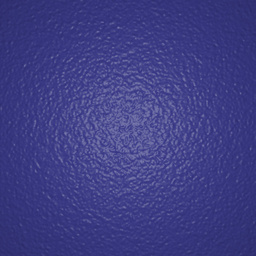
\includegraphics[width=\resLen]{bayesian/fig3/bump04rd1.jpg} &
		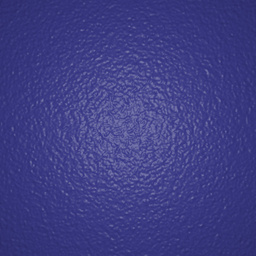
\includegraphics[width=\resLen]{bayesian/fig3/bump04rd2.jpg} &
		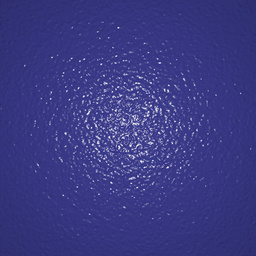
\includegraphics[width=\resLen]{bayesian/fig3/bump02rd1.jpg} &
		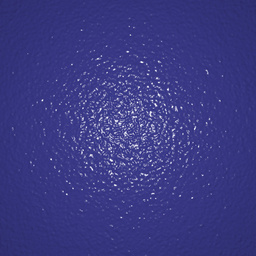
\includegraphics[width=\resLen]{bayesian/fig3/bump02rd2.jpg} \\
		(a1) & (a2) & (b1) & (b2)
	\end{tabular}
	\caption[L2 norm difference]{\label{fig:bayesian:sum_func}
		\textbf{L2 norm difference.} Each pair of images among (a, b) are generated using identical model parameters $\bmtheta$ but different irregularities $\bmz$. The pixel-wise L2 norm of the difference between these image pairs is large and not useful for estimating model parameters.
	}
\end{figure}

To overcome this challenge, we use the concept of a \emph{summary function}, which abstracts away the unimportant differences in the placement of the features, and summarizes the predicted and target images into smaller vectors whose similarity can be judged with simple metrics like L2 distance.

We define an image summary function $\summ$ to be a continuous function that maps an image of a material ($\target$ or $\synth$) into a vector in $\Reals^k$. An idealized summary function would have the property that
%
\begin{equation}
	\summ(f(\btheta_1, \bz_1)) = \summ(f(\btheta_2, \bz_2)) \ \Leftrightarrow \ \btheta_1 = \btheta_2.
\end{equation}
%
That is, applying the summary function would %fully
abstract away from the randomness $\bz$ and the difference between the two summary vectors would be entirely due to different material properties $\btheta$. Practical summary functions will satisfy the above only approximately. However, a good practical summary function will embed images of the same material close to each other, and images of different materials further away from each other. Below we discuss several techniques for constructing summary functions.

\paragraph*{Neural summary function.}
Gatys et al. \cite{Gatys2015,Gatys2016} introduced the idea of using the features of an image classification neural network (usually VGG \cite{VGG}) as a descriptor $T_G$ of image texture (or style). Optimizing images to minimize the difference in $T_G$ (combined with other constraints) allowed Gatys et al. to produce impressive, state-of-the art results for parametric texture synthesis and style transfer between images. While further work  has introduced improvements \cite{Risser2017}, we find that the original version from Gatys et al. works already well in our case.

Aittala et al. \cite{Aittala2016} introduced this technique to capturing material parameter textures (albedo, roughness, normal and specular maps) of stationary materials. They optimized for a $256 \times 256$ stationary patch that matches the target image in various crops, using a combination of $T_G$ and a number of special Fourier-domain priors. In our case (for procedural materials), we find that the neural summary function $T_G$ works even more effectively; we can simply apply it to the entire target or simulated images (not requiring crops nor Fourier-domain priors).
%
Specifically, define the Gram matrix $G$ of a set of feature maps $F_1, \cdots, F_n$ such that it has elements
\begin{equation}
	G_{ij} = \mbox{mean}(F_i \cdot F_j),
\end{equation}
where the product $F_i \cdot F_j$ is element-wise. $T_G$ is defined as the concatenation of the flattened Gram matrices computed for the feature maps before each pooling operation in VGG19. Note that the size of the Gram matrices depends on the number of feature maps (channels), not their size; thus $T_G$ is independent of input image size.

\label{ssec:example_summary_func}

\paragraph*{Statistics and Fourier transforms of image bins.}
While the neural summary function performs quite well, we find that in some cases we can improve upon it.
A simple idea for a summary function is to use the (RGB) mean of the entire image; an improvement is to subdivide the image into $k$ bins (regions) and compute the mean of each region. We found concentric bins perform well for isotropic materials, and vertical bins are appropriate for anisotropic highlights (e.g. brushed metal). Furthermore, we can additionally use a fast Fourier transform of the entire image or within bins. Note that automatic computation of derivatives is possible with the FFT, and supported by the PyTorch framework. In our current results, we use a summary function that combines the means and 1D FFTs of 64 vertical bins for the brushed metal example; all other examples use the neural summary function combined with simple image mean.


% \input{result_sumfunc}